This section describes the experimental approach followed to investigate the potential of Large Language Models (\llm{}s) in determining the suitability of a method for \textit{extract method} refactoring.

\begin{figure*}
\centering
%\noindent
\centerline{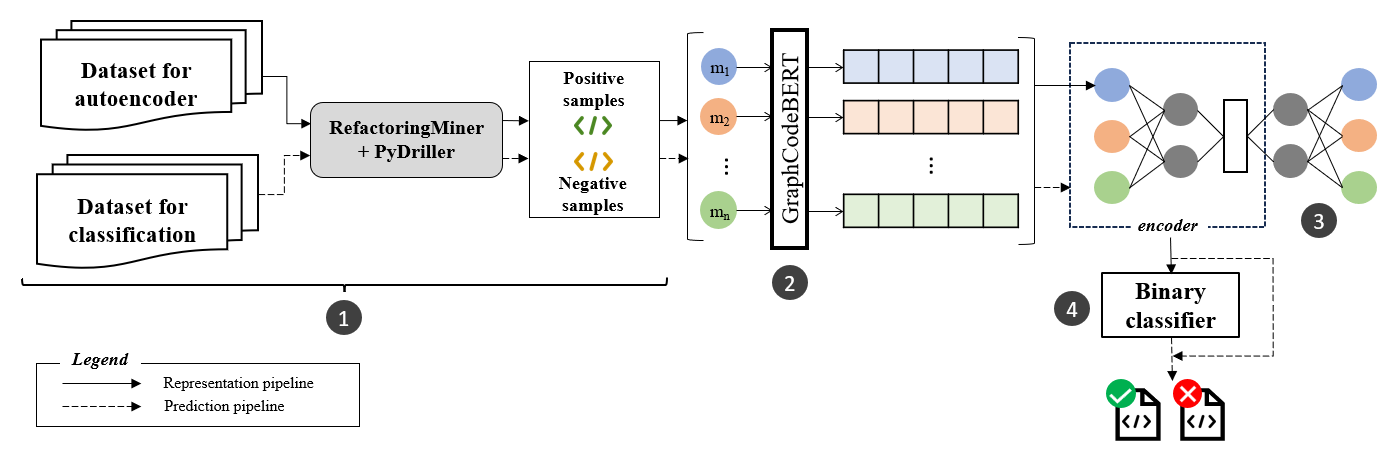
\includegraphics[width=\textwidth]{chapters/identification/Images/ArchDiagram.png}}
\caption{Overview of the proposed approach}
\label{fig:methodology}
% \vspace{-5pt}
\end{figure*}
\subsection{Overview}
The study aims to develop a \dl{}-based \exm{} refactoring candidate identification technique that addresses the deficiencies in the existing studies.
Figure~\ref{fig:methodology} presents an overview of our approach.
We first pick a set of repositories to prepare our dataset.
We use existing tools RefactoringMiner~\cite{Tsantalis:ICSE:2018:RefactoringMiner} and PyDriller~\cite{Spadini2018}, to segregate methods into positive and negative samples.
Our approach utilizes \GCB{} to generate embeddings for each sample.
We employ a \dl{} model based on Autoencoder~\cite{Liou2014Autoencoder} that is used for feature extraction and dimensionality reduction. 
We utilize the encoder component of the trained Autoencoder to generate a lower-dimensional latent space representation from the initially high-dimensional embedding input. 
The representation obtained from the bottleneck layer of Autoencoder is then used as a feature vector to train a \rf{} (\RF{}) classifier on the \exm{} identification task.
We formulate the following research questions.
% to evaluate the effectiveness of the proposed approach. 


\begin{itemize}
    \item [\textbf{RQ1}] 
    \textit{How does our proposed approach perform compared to the state-of-the-art?}
    % \smallskip
\end{itemize}    

    By answering this research question, we intend to evaluate and validate the performance of the proposed approach as compared to the
    % \todo{added -}
    state of the art. 


    \begin{itemize}
    \item 
    [\textbf{RQ2}] \textit{How effectively does the autoencoder extracts features for the classification task?}
\end{itemize}    
    In this research question,
    we aim to evaluate the effectiveness of the employed autoencoder-based model by extracting the learned features and using them for the classification task.


\subsection{Dataset preparation}
\label{dataset_prep}

We utilized a subset of repositories ($5$\%) from the $11,149$ open-source Java repositories used by Aniche~\etal{}~\cite{Aniche2020Effectiveness}, as working with the entire set required extensive computing infrastructure. This initial selection yielded $558$ repositories, from which we excluded repositories that were no longer available on GitHub or lacked any instances of \exm{} refactoring throughout their history. After filtering, we obtained $410$ repositories with at least one \exm{} refactoring performed. 
To leverage a trained autoencoder and using the trained encoder of the autoencoder for the classification task without data leakage, we divided this dataset into two parts: one for autoencoder pipeline with $208$ repositories and the remaining $202$ for the classification pipeline.



% \subsubsection{Dataset preparation}
As shown in step~\circled{1} of Figure~\ref{fig:methodology},
we use RefactoringMiner, a state-of-the-art refactoring detection tool~\cite{Tsantalis:ICSE:2018:RefactoringMiner, Tsantalis:TSE:2020:RefactoringMiner2.0} to prepare our dataset.
This tool reports performed refactorings, if any, 
in each commit within a Java repository's history. 
It provides essential metadata such as the code component involved (\eg{} method start line and end line in the case of \exm{} refactoring) and the associated commit hash. Leveraging this information, we utilize PyDriller~\cite{Spadini2018} to iterate through the identified commits and extract source code of the involved methods.


We identify positive samples where \exm{} refactoring has been applied following the mechanism described above.
Identifying negative samples for \exm{} refactoring is a challenging task. Merely excluding methods not reported by RefactoringMiner is insufficient since the absence of refactoring does not guarantee a method is not a refactoring candidate. Previous work have proposed heuristics-based approaches to address this challenge. For instance, Aniche~\etal{}~\cite{Aniche2020Effectiveness} used a criterion based on the method's modification history, while Yamanaka~\etal{}~\cite{Yamanaka2021RecommendingEM} selected code portions that differ from actual extractions. 
However, these heuristics may introduce noise and create sub-optimal datasets by misclassifying potential \exm{} candidates.

We propose a new mechanism to identify negative samples for the study. A method is considered a negative sample in commit $C_{n}$ if it underwent \exm{} refactoring in its parent commit $C_{n-1}$.  
The rationale behind this idea is that it is highly unlikely that a method that underwent \exm{} refactoring will again go through the same refactoring. This reduces the risk of false negative detection and ensures a high quality dataset. 
The aforementioned approach of identifying positive and negative samples, resulted in $27\small,634$ and $27\small,796$ samples for training and evaluating the Autoencoder, and  binary classifier respectively. Table~\ref{tab:ident_dataset_stats} describes the dataset statistics used to train, test and validate our approach.

\begin{table}[ht!]
    \centering
    \caption{Dataset statistics} \label{tab:ident_dataset_stats}
        \begin{tabular}{cccc|cccc}
            \toprule
            \multirow{2}{*}{Dataset} & \multicolumn{3}{c}{Positive samples} & \multicolumn{3}{c}{Negative samples} \\
            \cmidrule(lr){2-7}
& \makecell[c]{Avg.\\ LOC} &  \makecell[c]{Avg. \\ token\\ length} &  \makecell[c]{Median \\ LOC} &  \makecell[c]{Avg.\\ LOC} &  \makecell[c]{Avg.\\ token\\ length} &  \makecell[c]{Median \\ LOC} &\\
            \cmidrule(lr){1-7}
\makecell[l]{Train split}& $36.46$ & $343.26$ & $14$ & $26$ & $25.23$ & $263.24$\\ \addlinespace
\makecell[l]{Test split} & $36.22$ & $341.57$ & $14$ & $26$ & $24.46$ & $261.55$ \\ \addlinespace
\makecell[l]{Val split} & $35.57$ & $338.88$ & $13$ & $26$ & $25.50$ & $268.27$ \\ \addlinespace
% \makecell[l]{$\mathcal{D}$} & 411.68 & 447.69 & 185.94 & 241.88 \\ 
            \bottomrule
        \end{tabular}    
\end{table}
\vspace*{\fill}


\subsection{Data representation}

In step~\circled{2}, we use \GCB{} to capture both syntactic and semantic information of code, providing a comprehensive representation of code snippets by using graph-guided masked attention function to incorporate the code structure. 
The initial step in processing the input code through the \GCB{} model involves tokenization and encoding. To accomplish this, we utilize the pre-trained \GCB{} tokenizer.
% The \GCB{} model anticipates an input sequence of tokens, which must begin with a special \texttt{[CLS]} token and conclude with another special token, \texttt{[SEP]}. 
To ensure the token sequence adheres to the model's maximum length of $512$, we truncate it if it surpasses this limit. 
Subsequently, we perform batch encoding on the token sequence, generating \texttt{input\_ids} which represent the tokens numerically for the model. 

To extract the embeddings, we pass this encoded input to \GCB{}. 
During the forward propagation of the input, each of the $12$ hidden layers of the model generates individual token embeddings based on the surrounding context. To get the condensed representation of the sequence of tokens, we use mean pooling. We conducted a pilot study and we found that this approach performs better than taking the embedding of the \texttt{[SEP]} token alone.
This results in a single embedding vector of size $768$ for each of the input sample. We consider this as our feature vector for the classification task.

% \vspace{-1mm}

\subsection{Model training and classification}


\subsubsection{Autoencoder}

We use the generated embeddings from \GCB{} as the input for training the autoencoder model (step~\circled{3}). 
The architecture of the autoencoder that we trained consists of an encoder with three fully connected linear layers and ReLU activation to learn the hidden representation that reduces the input dimension to a bottleneck layer of size $128$. The decoder reverses this process to reconstruct the original input of size $768$. The autoencoder model is trained on $70\%$. The rest $30\%$ is used to validate the model. We calculate the reconstruction loss using \textit{Mean Squared Error} (MSE) loss.


\subsubsection{Binary classifier}
After training the autoencoder, in step~\circled{4}, we take the \textit{encoder} part of the trained model and use it as our feature extractor for the binary classification dataset.
We train two classifiers---a traditional machine learning model \rf{} and a \dl{}-based feed forward neural network, and compare their performance. 
We chose to use \rf{}
due to its ensemble learning method for classification and its ability to learn the non-linear relationship between the features,
\rf{} has shown to perform very well in different software engineering tasks~\cite{DiNucci2018, Immaculate2019} including refactoring identification~\cite{Aniche2020Effectiveness,VanDerLeij2021Data}. 

To train our models, 
we first split the $27,796$ samples into train, validation, and test sets in $70:10:20$ ratio 
using stratified sampling. 
We use \textit{GridSearchCV}
to select the optimal hyper-parameters for \rf{}.
The optimal set of hyper-parameter values along with their search space is reported in Table~\ref{tab:rfparams}
The neural network classifier consists of two fully connected layers with ReLU activation and a final sigmoid activation layer.

\begin{table*}[ht]
\captionsetup{skip=10pt}
\centering
\caption{Optimal hyper-parameter values for random forest}
\label{tab:rfparams}
\rowcolors{2}{gray!25}{white}
\begin{tabular}{p{5cm}%
>{\raggedleft\arraybackslash}p{4cm}%
>{\raggedleft\arraybackslash}p{4cm}%
}
\textbf{Parameter} & \textbf{Search space} & \textbf{Best value} \\ \midrule
Number of trees & ${[}100, 200, 300, 1000{]}$ & $1000$ \\
Minimum samples split    & ${[}8, 10, 12{]}$           & $10$   \\
Minimum leaf node samples              & ${[}3, 4, 5{]}$             & $3$    \\
Maximum features              & ${[}2, 3{]}$                & $2$    \\
Maximum tree depth                    & ${[}80, 90, 100, 110{]}$    & $80$  \\\bottomrule
% \vspace{-5pt}
\end{tabular}
\end{table*}

\subsubsection{Evaluation}

To evaluate our models, we calculate the \textit{accuracy, precision, recall,} and \textit{F1 score}.


Initially, the test split of our classification dataset, 
contains positive and negative samples in equal proportion. 
However, it has been argued~\cite{Sharma2021, DiNucci2018} that a test set not representative of the real-world may show good performance while experimentation 
but do poorly when deployed in a real-world scenario. 
To address this issue, 
we identify the ratio of positive and negative samples in the following manner. 
First, we sample $20$ repositories from our dataset randomly. 
For each of the selected repositories, we identify the commits in which \exm{} refactoring has been applied using RefactoringMiner along with the count of such methods ($posCount$). 
Using PyDriller, we identify the count of total methods present in the source code for that commit ($totalCount$). 
Then we compute the ratio $\frac{posCount}{totalCount}$ and take the mean across all identified commits to find a real-world ratio of \exm{} refactoring candidates. 
We modify the test set  to represent the computed ratio ($85:15$) and then perform the evaluation. 
